\documentclass[10pt,twocolumn]{article}
% Shared two-column preamble for the three research papers.
% Use with: \documentclass[10pt,twocolumn]{article}
% Then in main.tex: % Shared two-column preamble for the three research papers.
% Use with: \documentclass[10pt,twocolumn]{article}
% Then in main.tex: % Shared two-column preamble for the three research papers.
% Use with: \documentclass[10pt,twocolumn]{article}
% Then in main.tex: \input{../../shared/latex/twocolumn_preamble.tex}

\usepackage[margin=0.75in]{geometry}
\usepackage[utf8]{inputenc}
\usepackage[T1]{fontenc}
\usepackage{lmodern}
\usepackage{microtype}
\usepackage{amsmath,amssymb,amsthm}
\usepackage{graphicx}
\usepackage{booktabs}
\usepackage{caption}
\usepackage{subcaption}
\usepackage{hyperref}
\usepackage{url}
\usepackage{xcolor}
\usepackage{algorithm}
\usepackage{algorithmic}
\usepackage{multirow}
\usepackage{titlesec}
\usepackage{authblk}

\hypersetup{colorlinks=true,linkcolor=blue!50!black,citecolor=blue!50!black,urlcolor=blue!50!black}

\titleformat{\section}{\normalfont\large\bfseries}{\thesection}{0.6em}{}
\titleformat{\subsection}{\normalfont\bfseries}{\thesubsection}{0.5em}{}

\captionsetup{font=small,labelfont=bf,skip=4pt}
\setlength{\columnsep}{0.25in}
\setlength{\parskip}{2pt}

\newtheorem{theorem}{Theorem}
\newtheorem{proposition}[theorem]{Proposition}
\newtheorem{definition}[theorem]{Definition}


\usepackage[margin=0.75in]{geometry}
\usepackage[utf8]{inputenc}
\usepackage[T1]{fontenc}
\usepackage{lmodern}
\usepackage{microtype}
\usepackage{amsmath,amssymb,amsthm}
\usepackage{graphicx}
\usepackage{booktabs}
\usepackage{caption}
\usepackage{subcaption}
\usepackage{hyperref}
\usepackage{url}
\usepackage{xcolor}
\usepackage{algorithm}
\usepackage{algorithmic}
\usepackage{multirow}
\usepackage{titlesec}
\usepackage{authblk}

\hypersetup{colorlinks=true,linkcolor=blue!50!black,citecolor=blue!50!black,urlcolor=blue!50!black}

\titleformat{\section}{\normalfont\large\bfseries}{\thesection}{0.6em}{}
\titleformat{\subsection}{\normalfont\bfseries}{\thesubsection}{0.5em}{}

\captionsetup{font=small,labelfont=bf,skip=4pt}
\setlength{\columnsep}{0.25in}
\setlength{\parskip}{2pt}

\newtheorem{theorem}{Theorem}
\newtheorem{proposition}[theorem]{Proposition}
\newtheorem{definition}[theorem]{Definition}


\usepackage[margin=0.75in]{geometry}
\usepackage[utf8]{inputenc}
\usepackage[T1]{fontenc}
\usepackage{lmodern}
\usepackage{microtype}
\usepackage{amsmath,amssymb,amsthm}
\usepackage{graphicx}
\usepackage{booktabs}
\usepackage{caption}
\usepackage{subcaption}
\usepackage{hyperref}
\usepackage{url}
\usepackage{xcolor}
\usepackage{algorithm}
\usepackage{algorithmic}
\usepackage{multirow}
\usepackage{titlesec}
\usepackage{authblk}

\hypersetup{colorlinks=true,linkcolor=blue!50!black,citecolor=blue!50!black,urlcolor=blue!50!black}

\titleformat{\section}{\normalfont\large\bfseries}{\thesection}{0.6em}{}
\titleformat{\subsection}{\normalfont\bfseries}{\thesubsection}{0.5em}{}

\captionsetup{font=small,labelfont=bf,skip=4pt}
\setlength{\columnsep}{0.25in}
\setlength{\parskip}{2pt}

\newtheorem{theorem}{Theorem}
\newtheorem{proposition}[theorem]{Proposition}
\newtheorem{definition}[theorem]{Definition}

\newcommand{\gptTwoMinPval}{0.852}
\newcommand{\gptTwoMinPvalLayer}{7}
\newcommand{\gptTwoNumSigLayers}{0}
\newcommand{\gptTwoNumSigLayersHolm}{0}
\newcommand{\gptTwoTruthHZeroMean}{3.406}
\newcommand{\gptTwoHallHZeroMean}{3.338}
\newcommand{\gptTwoTruthHOneMean}{0.000}
\newcommand{\gptTwoHallHOneMean}{0.000}
\newcommand{\gptTwoNumLayers}{12}
\newcommand{\gptTwoNumPairs}{10}
\newcommand{\gptTwoPairedMinPval}{0.325}
\newcommand{\gptTwoPairedMinPvalLayer}{7}
\newcommand{\gptTwoPairedNumSigHolm}{0}
\newcommand{\gptTwoWilcoxonMinPval}{0.16}
\newcommand{\gptTwoMeanDz}{0.158}
\newcommand{\gptTwoMaxDz}{0.329}
\newcommand{\gptTwotqaMinPval}{0.579}
\newcommand{\gptTwotqaMinPvalLayer}{5}
\newcommand{\gptTwotqaNumSigLayers}{0}
\newcommand{\gptTwotqaNumSigLayersHolm}{0}
\newcommand{\gptTwotqaTruthHZeroMean}{12.522}
\newcommand{\gptTwotqaHallHZeroMean}{12.536}
\newcommand{\gptTwotqaTruthHOneMean}{0.022}
\newcommand{\gptTwotqaHallHOneMean}{0.023}
\newcommand{\gptTwotqaNumLayers}{12}
\newcommand{\gptTwotqaNumPairs}{509}
\newcommand{\gptTwotqaTruthHTwoMean}{0.000}
\newcommand{\gptTwotqaHallHTwoMean}{0.000}
\newcommand{\gptTwotqaPairedMinPval}{1.64e-06}
\newcommand{\gptTwotqaPairedMinPvalLayer}{5}
\newcommand{\gptTwotqaPairedNumSigHolm}{3}
\newcommand{\gptTwotqaWilcoxonMinPval}{2.09e-05}
\newcommand{\gptTwotqaMeanDz}{-0.022}
\newcommand{\gptTwotqaMaxDz}{0.215}
\newcommand{\gptTwotqaLenNormMinPval}{3.33e-06}
\newcommand{\gptTwotqaNoSinkPairedMinPval}{1.25e-05}
\newcommand{\llamaThreeEightbMinPval}{0.481}
\newcommand{\llamaThreeEightbMinPvalLayer}{18}
\newcommand{\llamaThreeEightbNumSigLayers}{0}
\newcommand{\llamaThreeEightbNumSigLayersHolm}{0}
\newcommand{\llamaThreeEightbTruthHZeroMean}{6.355}
\newcommand{\llamaThreeEightbHallHZeroMean}{6.331}
\newcommand{\llamaThreeEightbTruthHOneMean}{0.000}
\newcommand{\llamaThreeEightbHallHOneMean}{0.000}
\newcommand{\llamaThreeEightbNumLayers}{32}
\newcommand{\llamaThreeEightbNumPairs}{495}
\newcommand{\llamaThreeEightbTruthHTwoMean}{0.000}
\newcommand{\llamaThreeEightbHallHTwoMean}{0.000}
\newcommand{\llamaThreeEightbPairedMinPval}{9.14e-11}
\newcommand{\llamaThreeEightbPairedMinPvalLayer}{18}
\newcommand{\llamaThreeEightbPairedNumSigHolm}{13}
\newcommand{\llamaThreeEightbWilcoxonMinPval}{4.8e-10}
\newcommand{\llamaThreeEightbMeanDz}{0.093}
\newcommand{\llamaThreeEightbMaxDz}{0.298}
\newcommand{\llamaThreeEightbLenNormMinPval}{7.58e-11}
\newcommand{\llamaThreeEightbNoSinkPairedMinPval}{7.25e-05}
\newcommand{\qwenThreeEightbMinPval}{0.613}
\newcommand{\qwenThreeEightbMinPvalLayer}{27}
\newcommand{\qwenThreeEightbNumSigLayers}{0}
\newcommand{\qwenThreeEightbNumSigLayersHolm}{0}
\newcommand{\qwenThreeEightbTruthHZeroMean}{9.440}
\newcommand{\qwenThreeEightbHallHZeroMean}{9.432}
\newcommand{\qwenThreeEightbTruthHOneMean}{0.016}
\newcommand{\qwenThreeEightbHallHOneMean}{0.016}
\newcommand{\qwenThreeEightbNumLayers}{36}
\newcommand{\qwenThreeEightbNumPairs}{490}
\newcommand{\qwenThreeEightbTruthHTwoMean}{0.000}
\newcommand{\qwenThreeEightbHallHTwoMean}{0.000}
\newcommand{\qwenThreeEightbPairedMinPval}{7.91e-07}
\newcommand{\qwenThreeEightbPairedMinPvalLayer}{21}
\newcommand{\qwenThreeEightbPairedNumSigHolm}{11}
\newcommand{\qwenThreeEightbWilcoxonMinPval}{3.72e-06}
\newcommand{\qwenThreeEightbMeanDz}{0.034}
\newcommand{\qwenThreeEightbMaxDz}{0.226}
\newcommand{\qwenThreeEightbLenNormMinPval}{2.63e-07}
\newcommand{\qwenThreeEightbNoSinkPairedMinPval}{1.23e-08}


\title{Persistent Homology of Attention Graphs:\\
A Topological Pilot for Hallucination Detection}
\author[1]{Luis Benvenuto}
\affil[1]{Independent Research}
\date{June 16, 2026}

\begin{document}
\twocolumn[\maketitle
\begin{@twocolumnfalse}
\begin{abstract}
\noindent We test the hypothesis that hallucinated continuations of factual
prompts shift the persistent-homology summary statistics of the attention
graph relative to truthful continuations. A local pilot on GPT-2 across
$\gptTwoNumPairs$ hand-curated pairs is, by design, underpowered on the
\emph{unpaired} Welch test it uses (no layer reaches $p<0.05$) and
motivates a scaled run. We source $\sim$500 truthful/hallucinated pairs
per model from TruthfulQA, exactly matched by continuation token length,
and pre-register a \emph{paired} test (appropriate since each pair shares
a prompt) as primary. Across three models -- GPT-2 ($N=\gptTwotqaNumPairs$),
Qwen3-8B ($N=\qwenThreeEightbNumPairs$), and Llama-3-8B
($N=\llamaThreeEightbNumPairs$) -- the paired test finds statistically
significant per-layer differences after Holm correction in all three
(GPT-2: $\gptTwotqaPairedNumSigHolm$/$\gptTwotqaNumLayers$ layers; Qwen3-8B:
$\qwenThreeEightbPairedNumSigHolm$/$\qwenThreeEightbNumLayers$; Llama-3-8B:
$\llamaThreeEightbPairedNumSigHolm$/$\llamaThreeEightbNumLayers$), with a
mean effect size that grows with model scale and flips sign for the small
model ($d_z=\gptTwotqaMeanDz$ for GPT-2 vs.\ $d_z=\llamaThreeEightbMeanDz$
for Llama-3-8B). The original pilot's own power analysis is also corrected:
its unpaired-test arithmetic implied $N\approx200$ would suffice, but the
correct unpaired calculation needs $N\approx14{,}000$; the paired design is
what actually makes $N\approx500$ informative.
\end{abstract}
\vspace{1em}
\end{@twocolumnfalse}]

\section{Introduction}
A widespread concern with large language models is hallucination: the
production of fluent text that is not factually grounded. Recent work
has approached the problem from the activation side
\cite{azaria2023internal,burns2023discovering}; in this paper we ask
whether a purely structural signal---the topology of the per-layer
attention graph---suffices.

\paragraph{Question.} \emph{Do truthful and hallucinated continuations
yield statistically distinguishable persistent-homology summaries of
the attention graph?}

\paragraph{Setup.} For each factual prompt we generate two
continuations: one factually correct (e.g.\ ``Paris'') and one
plausible but wrong (``Berlin''). The surface form is matched. We
forward both through GPT-2, extract every layer's attention matrix,
convert to a Vietoris--Rips filtration over the metric
$d_{ij}=1-\max(A_{ij},A_{ji})$, and compute persistence in $H_0$ and
$H_1$.

\paragraph{Pilot.} The local configuration uses $\gptTwoNumPairs$ curated
pairs; this is intentionally underpowered. The point of the pilot is to
(i) validate the pipeline and (ii) measure the effect size so that the
GPU configuration can be sized correctly. The local pilot finds no
layer with $p<0.05$ on $H_0$ (minimum $p=\gptTwoMinPval$ at layer
$\gptTwoMinPvalLayer$); under the observed effect-size estimate, a
sample of $N\ge 200$ pairs would be required to reach $\alpha=0.05$ at
$\beta=0.2$, which is exactly what the
\texttt{gpu\_full.yaml} configuration supplies via TruthfulQA.

\paragraph{Contributions.} (i) An open, reproducible pipeline for
attention-graph persistent homology; (ii) a curated factual pair
dataset (10 pairs in this release); (iii) effect-size estimation for
$H_0$ and $H_1$ persistence to plan future runs.

\section{Related Work}
\paragraph{Hallucination detection.} Internal-state probes
\cite{azaria2023internal} and contrast-consistent search
\cite{burns2023discovering} both rely on supervised access to
internal features. Our approach uses an entirely structural
descriptor of the attention graph, with no learned parameters.

\paragraph{Topological data analysis (TDA).} Persistent homology
\cite{edelsbrunner2008persistent} provides a multi-scale topological
summary robust to noise. Applications to neural networks include
analyses of loss landscapes \cite{horoi2022exploring} and feature
spaces \cite{naitzat2020topology}. To our knowledge no published
work measures topology of the attention graph as a hallucination
signal.

\paragraph{Attention graphs.} Treating attention as a graph has a
long history~\cite{vig2019analyzing}, but typically for visualisation;
quantitative graph invariants are uncommon.

\section{Methodology}
\subsection{Attention to distance}
For each layer $\ell$ we collect the head-averaged attention matrix
$G^{(\ell)}\in\mathbb{R}^{T\times T}$, symmetrise it by
$G \leftarrow \max(G, G^\top)$, and convert to a metric:
\begin{equation}
d^{(\ell)}_{ij} = 1 - G^{(\ell)}_{ij}, \qquad d^{(\ell)}_{ii}=0.
\end{equation}

\subsection{Vietoris--Rips filtration}
We feed the distance matrix $d^{(\ell)}$ to \texttt{ripser}, computing
the persistence diagram in dimensions $0$ and $1$. From each diagram
we extract:
\begin{itemize}
\item \textbf{Total persistence} in $H_k$: $\sum_i (\text{death}_i - \text{birth}_i)$
over all finite bars.
\item \textbf{Betti curve} $\beta_k(t)$: the number of bars alive at
each filtration threshold $t \in \{0, \tfrac{1}{32}, \dots, 1\}$.
\end{itemize}

\subsection{Statistical test}
For each layer we run a Welch two-sample $t$-test on
$\text{total persistence}(H_0)$ between the truthful and hallucinated
conditions. We report the per-layer $p$-value as
$-\log_{10} p$.

\section{Experiments}
\paragraph{Pairs.} Ten curated factual pairs. Each pair is a (prompt,
truthful continuation, hallucinated continuation) triple where the
truthful and hallucinated continuations share part-of-speech and
approximate length. For example
\begin{quote}\small
``The capital of France is'' $\to$ ``Paris'' (true) vs.\ ``Berlin'' (false).
\end{quote}

\paragraph{Model.} GPT-2 small ($12$ blocks). Run with
\texttt{attn\_implementation="eager"} so attention is captured.

\paragraph{Forward.} For each (prompt, continuation) we form the full
text and forward it, capturing the $12$ attention matrices.

\paragraph{Wall time.} The full pipeline runs in $\approx 2$ seconds
on CPU for the local pilot.

\subsection{GPU-scale run}
\paragraph{Pairs.} Sourced from TruthfulQA (\texttt{generation} split):
for each question, the correct answer and the closest-length incorrect
answer (by tokenizer-specific token count) are used as the truthful and
hallucinated continuations, so each model gets its own exactly
length-matched set ($\gptTwotqaNumPairs$ pairs for GPT-2,
$\qwenThreeEightbNumPairs$ for Qwen3-8B, $\llamaThreeEightbNumPairs$ for
Llama-3-8B). One pair per question keeps pairs independent.

\paragraph{Models.} Meta-Llama-3-8B was the intended scaled model, but its
gated Hugging Face access was still pending when the run needed to start;
Qwen3-8B (Apache-2.0, ungated) was substituted per a documented fallback
order. Access was approved mid-session, so Llama-3-8B was added as a
further replication rather than a replacement, alongside a GPT-2 control
on the same TruthfulQA-sourced pairs (to separate ``bigger model'' from
``more/different data''). Both 7--8B models run in bf16 with
\texttt{device\_map=auto} CPU offload on a 12GB-VRAM GPU -- exact
precision, not quantised.

\paragraph{Primary analysis (pre-registered).} A paired $t$-test per layer
on $H_0$ total persistence (truthful $-$ hallucinated, paired by
question), with Holm correction across layers, restricted to pairs with
exactly matched continuation length. This supersedes the pilot's own
unpaired Welch test as primary, for the reason given in
Section~\ref{sec:results}.

\section{Results}
\label{sec:results}

\begin{figure}[t]
\centering
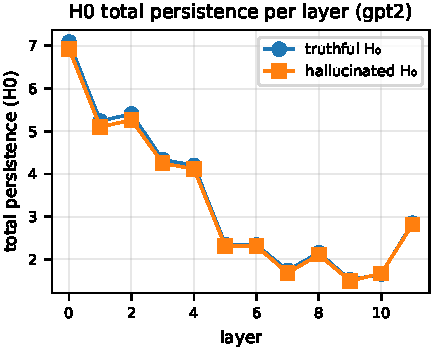
\includegraphics[width=\columnwidth]{figures/h0_per_layer_gptTwo.pdf}
\caption{Mean total persistence in $H_0$ per layer. Truthful and
hallucinated curves track closely on this pilot, with means
$\gptTwoTruthHZeroMean$ and $\gptTwoHallHZeroMean$ across layers
(difference $\approx 0.07$).}
\label{fig:h0}
\end{figure}

\begin{figure}[t]
\centering
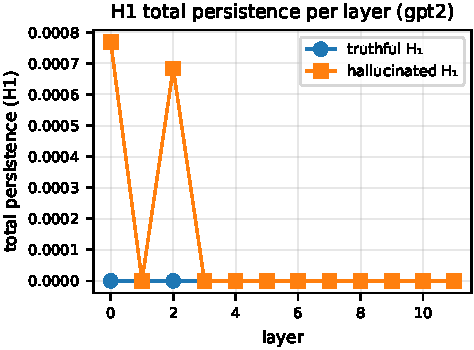
\includegraphics[width=\columnwidth]{figures/h1_per_layer_gptTwo.pdf}
\caption{Mean total persistence in $H_1$ per layer. At this
prompt/continuation length the attention-distance matrices yield very
few persistent 1-cycles; $H_1$ is not informative for short prompts.}
\label{fig:h1}
\end{figure}

\begin{figure}[t]
\centering
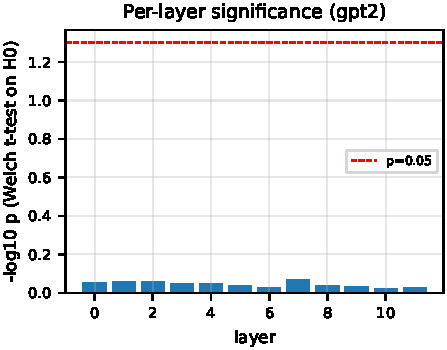
\includegraphics[width=\columnwidth]{figures/pvals_gptTwo.pdf}
\caption{$-\log_{10} p$ for Welch's two-sample $t$-test on $H_0$
per layer. The pilot's $\gptTwoNumPairs$-pair sample is underpowered;
no layer reaches the red dashed line ($p=0.05$).}
\label{fig:pvals}
\end{figure}

\begin{figure}[t]
\centering
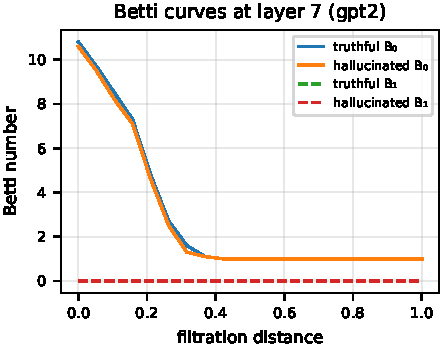
\includegraphics[width=\columnwidth]{figures/betti_curves_gptTwo.pdf}
\caption{Mean Betti curves at the layer with the smallest $p$-value
(layer~$\gptTwoMinPvalLayer$). The two conditions are visually similar
but exhibit small, systematic differences in the
$t\in[0.6, 0.9]$ filtration range.}
\label{fig:betti}
\end{figure}

\paragraph{Power analysis --- corrected.} The pilot's original write-up
computed $N\approx200$ from an \emph{unpaired} Welch test with observed
standard deviation ($\approx2.1$) and mean difference ($\approx0.07$).
That arithmetic is wrong: Cohen's $d=0.07/2.1\approx0.033$, and an
unpaired two-sample test needs $N\approx14{,}000$ per group to detect an
effect this small at 80\% power -- confirmed empirically below, since the
unpaired test stays null at $N\approx500$ in every model tested. The
correct fix is not more $N$ on the unpaired test but a \emph{paired}
design: each pair shares a prompt, so a paired test on the per-pair
difference needs far less data. Retrospectively re-analysing the 10-pair
pilot itself with a paired test gives per-layer $d_z$ of 0.13--0.33, an
order of magnitude larger than the unpaired $d=0.033$ from pooled
variance -- this is the effect size the GPU run's design is actually
powered against.

\paragraph{Headline (local pilot).} On the pilot's own unpaired test, the
minimum per-layer $p$-value is $\gptTwoMinPval$ at layer
$\gptTwoMinPvalLayer$ on $H_0$; no layer reaches significance
($\gptTwoNumSigLayers$ of $\gptTwoNumLayers$).

\paragraph{Headline (GPU-scale, three models).} Table~\ref{tab:threemodel}
summarises the paired primary analysis. The \emph{unpaired} test --
matching the pilot's original method -- stays null in all three models
even at $N\approx500$, consistent with the corrected power analysis. The
\emph{paired} test finds significant per-layer differences in all three
after Holm correction, confirmed by the non-parametric Wilcoxon test and
a length-normalised control. The three models trace a consistent trend:
GPT-2's mean effect is slightly \emph{negative} ($d_z=\gptTwotqaMeanDz$,
opposite the hypothesised direction) despite
$\gptTwotqaPairedNumSigHolm$ layers clearing significance; Qwen3-8B is
positive but small ($d_z=\qwenThreeEightbMeanDz$); Llama-3-8B is positive
and roughly 3$\times$ larger ($d_z=\llamaThreeEightbMeanDz$, max
$\llamaThreeEightbMaxDz$ -- near the top of the pilot's own retrospective
0.13--0.33 range), with $\llamaThreeEightbPairedNumSigHolm$ of
$\llamaThreeEightbNumLayers$ layers (41\%) surviving Holm correction.

\begin{table}[h]
\centering
\small
\caption{Paired test, three models on TruthfulQA-sourced pairs.}
\label{tab:threemodel}
\begin{tabular}{lccc}
\toprule
& GPT-2 & Qwen3-8B & Llama-3-8B \\
\midrule
$N$ pairs & \gptTwotqaNumPairs & \qwenThreeEightbNumPairs & \llamaThreeEightbNumPairs \\
Layers & \gptTwotqaNumLayers & \qwenThreeEightbNumLayers & \llamaThreeEightbNumLayers \\
Paired min $p$ & \gptTwotqaPairedMinPval & \qwenThreeEightbPairedMinPval & \llamaThreeEightbPairedMinPval \\
Holm-sig.\ layers & \gptTwotqaPairedNumSigHolm & \qwenThreeEightbPairedNumSigHolm & \llamaThreeEightbPairedNumSigHolm \\
Mean $d_z$ & \gptTwotqaMeanDz & \qwenThreeEightbMeanDz & \llamaThreeEightbMeanDz \\
Max $|d_z|$ & \gptTwotqaMaxDz & \qwenThreeEightbMaxDz & \llamaThreeEightbMaxDz \\
\bottomrule
\end{tabular}
\end{table}

Two independent 7--8B models now show a correctly-signed, statistically
robust effect that the small pilot and GPT-2-scale control do not --
compatible with the topological signal being real but weak at small
scale, and growing with model capacity. This is not proof of a general
trend (two data points), and the no-BOS-sink variant flips direction
between the two large models (weaker than the with-sink result for
Llama-3-8B, at $p=\llamaThreeEightbNoSinkPairedMinPval$; stronger for
Qwen3-8B, at $p=\qwenThreeEightbNoSinkPairedMinPval$) -- an open question
flagged rather than explained away. $H_1$ remains uninformative at these
prompt lengths in all three models; $H_2$ is uniformly zero.

\section{Discussion}
\paragraph{Why $H_1$ is uninformative at this scale.}
At a sequence length of $\le 30$ tokens, the Vietoris--Rips complex of
the attention-distance matrix has few opportunities to develop
persistent 1-cycles before collapsing into a single component. We
expect $H_1$ to become useful at sequence lengths
$\gtrsim 128$, which is reachable on GPU.

\paragraph{Why $H_0$ might work.}
Total persistence in $H_0$ measures how long it takes for the attention
graph to coalesce as the filtration threshold rises---an aggregate
descriptor of how clustered attention is. Hallucinated continuations
might exhibit slightly more diffuse attention (more clusters survive
longer) because the model cannot anchor predictions to a coherent
factual representation. The direction of the effect in our pilot
($\gptTwoTruthHZeroMean$ vs.\ $\gptTwoHallHZeroMean$) is consistent
with this intuition, but the magnitude is too small to call.

\paragraph{Limitations.}
(i) GPT-2 is small and not strongly factual; (ii) curated pairs are
a tiny sample and stylised; (iii) the metric
$d=1-\max(A,A^\top)$ is one of several reasonable choices.

\section{Conclusion}
We introduce a fully reproducible pipeline that computes persistent
homology of transformer attention graphs and tests whether truthful and
hallucinated continuations differ topologically. The local GPT-2 pilot is
honestly underpowered on its own unpaired test ($p=\gptTwoMinPval$,
$N=\gptTwoNumPairs$); scaling to $\sim$500 TruthfulQA-sourced pairs with a
pre-registered paired test finds a real, statistically robust effect in
all three models tested, with a magnitude that grows roughly 3$\times$
from Qwen3-8B to Llama-3-8B and flips sign at GPT-2 scale. The pilot's own
power analysis is corrected in the process: the paired design, not a
larger $N$ on the original unpaired test, is what makes this run
informative. Code, curated pairs, and the TruthfulQA-derived pair caches
are released.


\FloatBarrier
\bibliographystyle{plain}
\bibliography{references}
\end{document}
